\section{Usage sample mining}
\label{sec:usage_mining}

\begin{figure*}
	\newcommand\lowlight[1]{\textcolor{gray}{#1}}
	\newcommand\highlight[1]{\textcolor{red}{#1}}
	\centering
	\begin{subfigure}[t]{.32\linewidth}
		\begin{tikzpicture}
	\node {CallExpression}
		child {node [accent1] {identifier}}
		child [gray] {node [gray, yshift = -0.5cm] {typeArguments}}
		child [gray] {node [gray] {arguments}};
\end{tikzpicture}
\caption[LoF entry]{
	Node pattern for a TypeScript functional call, such as in:

	\code{\textlowlight{result = }\uline{\texthighlight{fun}<\textlowlight{T1}, \textlowlight{T2}>(\textlowlight{arg1}, \textlowlight{arg2})}\textlowlight{;}}
}

	\end{subfigure}
	\hfill
	\begin{subfigure}[t]{.32\linewidth}
		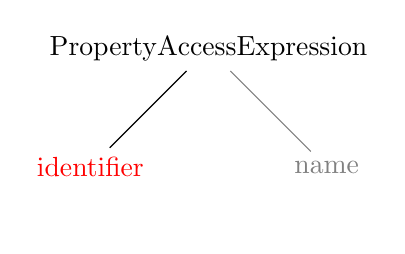
\begin{tikzpicture}
	\node {PropertyAccessExpression}
		child {node [red] {identifier}}
		child [white] {node [yshift = -0.5cm] {\phantom{node}}}  % ensure same height as sibling figures
		child [gray] {node [gray] {name}}
		;
\end{tikzpicture}
\caption[LoF entry]{
	Node pattern for a property access, such as in:

	\code{\lowlight{return }\uline{\lowlight{obj}.\highlight{prop}}\lowlight{;}}
}

	\end{subfigure}
	\hfill
	\begin{subfigure}[t]{.32\linewidth}
		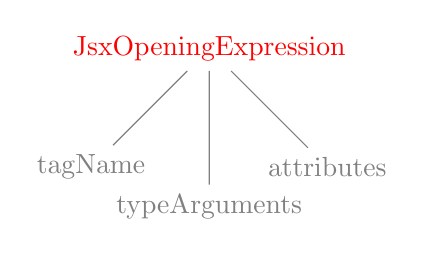
\begin{tikzpicture}
	\node [red] {JsxOpeningExpression}
		child [gray] {node [gray] {tagName}}
		child [gray] {node [gray, yshift = -0.5cm] {typeArguments}}
		child [gray] {node [gray] {attributes}};
\end{tikzpicture}
\caption[LoF entry]{
	Node pattern for a JSX opening element (as supported in React\protect\footnotemark{} or TypeScript\protect\footnotemark{}), such as in:
	\code{\lowlight{elem = }\uline{<Button \lowlight{color}="\lowlight{blue}"> \lowlight{Google</Button>}}\lowlight{;}}
}

	\end{subfigure}

	\caption{AST patterns for example JavaScript/TypeScript expressions.
		The \highlight{highlighted} node contains the link to the declaration of the referenced identifier.
	}
	\label{fig:usage_mining/patterns}
\end{figure*}
\addtocounter{footnote}{-1}
\footnotetext{\url{https://reactjs.org/docs/introducing-jsx.html}}
\addtocounter{footnote}{1}
\footnotetext{\url{https://www.typescriptlang.org/docs/handbook/jsx.html}}


Having downloaded the selected downstream dependency repositories, we can proceed to extract usage samples for the target package from each dependency repository.
Our goal is to identify these usage samples on a fine-granular level so that we can trace them down to the single identifiers that were exposed by the target package.

To do so, we start by parsing the source code of every dependency repository as well as the source of the target package each into a separate AST.

% TODO: use term "binding"?
In a second step, every dependency AST is traversed together with the target package AST in order to create links between semantically related nodes, e.g., between an expression and the variable it is assigned to or between a function call and the definition of this function.

In the final step, the AST is traversed again and collect all nodes that are linked to a declaration in the target package.
To identify these links, we define a set of language-specific patterns of AST subtrees that containing a declaration node (see \cref{fig:usage_mining/patterns}).
